\documentclass{article}
%\usepackage[superscript]{cite}
\usepackage[pdftex]{graphicx}
\usepackage{sidecap}
\usepackage{caption}
\usepackage{subcaption}
\usepackage{amsmath}
\usepackage{amsfonts}
\usepackage{tikz}
\usepackage{pgfplots}
\usepackage[colorlinks=true,linkcolor=blue,citecolor=blue]{hyperref}
\usepackage{fullpage}
%\usepackage{natbib}
\usepackage[utf8]{inputenc}
\usepackage[english]{babel}
\newcommand{\angstrom}{\text{\normalfont\AA}}


\begin{document}



\section{ONC Structure}
Here we specify the structure/hierarchy that exists for the ONC. At its highest level, we have three directories: \textbf{Tickets}, \textbf{JSON Files}, and \textbf{Individual Novae}. Let's start with the \textbf{Individual Novae} directory.


\begin{figure}[h]
\centering
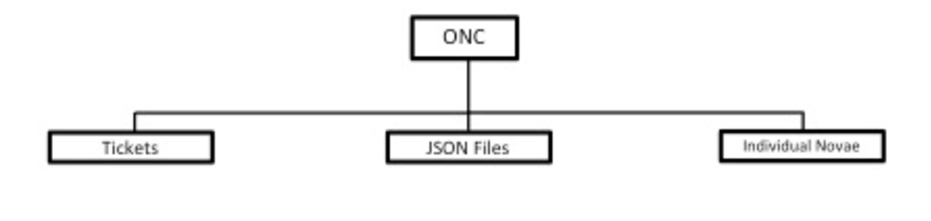
\includegraphics[width=15cm]{DataHierarchy_Pics/Pic1} 
%\caption{ }
%\label{fig:1}
\end{figure}

The \textbf{Individual Novae} directory is laid out in a modular fashion, such that each individual nova has its own directory for storing the data--as well as the tickets--associated with it. 


For example, let's take the nova FH Ser. 


\begin{figure}[h]
\centering
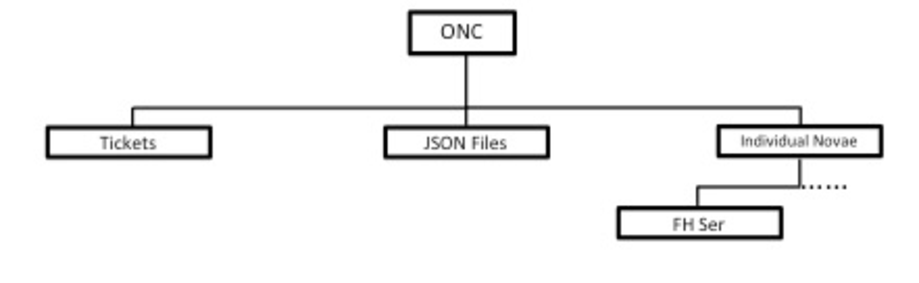
\includegraphics[width=15cm]{DataHierarchy_Pics/Pic2} 
%\caption{ }
%\label{fig:2}
\end{figure}


Within the FH Ser directory we have sub-directories for the tickets that are--or will be--generated for FH Ser; we also have a directory for the data that has been--or will be--collected for FH Ser. Finally, this directory is also where the JSON file for FH Ser will/does live.


\begin{figure}[h]
\centering
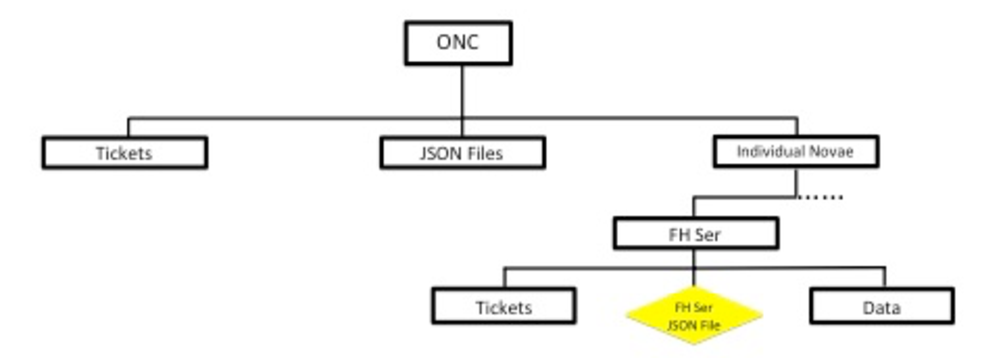
\includegraphics[width=15cm]{DataHierarchy_Pics/Pic3} 
%\caption{ }
%\label{fig:3}
\end{figure}


Looking at the tickets directory, we see that there are two sub-directories within it: \emph{Pending Tickets} and \emph{Completed Tickets}. We have examples of completed tickets within these directories as well; one is a (completed) radio photometry ticket, and the other is a (pending) optical photometry ticket. 


\begin{figure}[h]
\centering
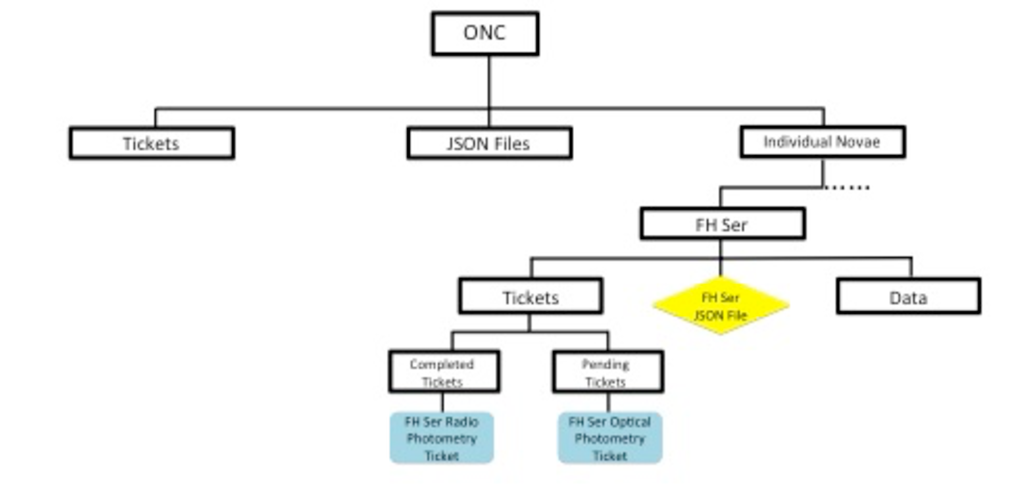
\includegraphics[width=15cm]{DataHierarchy_Pics/Pic4} 
%\caption{ }
%\label{fig:4}
\end{figure}

We will only build the JSON file using completed tickets. 

A completed ticket means that we must have gotten some piece of data for this nova. Where does that data live? In the data directory.


\begin{figure}[h]
\centering
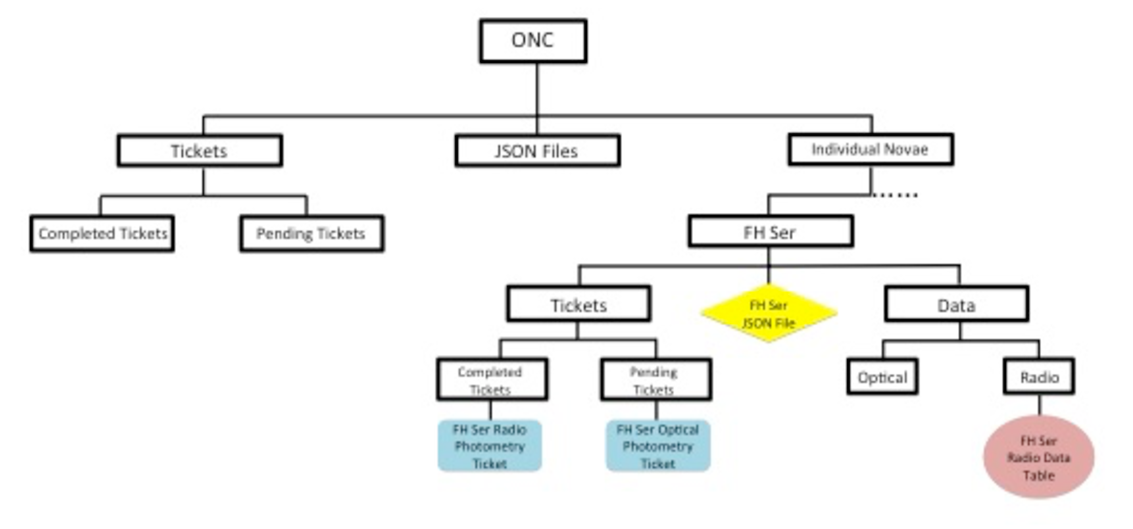
\includegraphics[width=15cm]{DataHierarchy_Pics/Pic5} 
%\caption{ }
%\label{fig:5}
\end{figure}

The data directory stores all of the data that we have accumulated for this particular nova. As you can see, it's subdivided by wavelength regime.


Finally, as mentioned previously, this is the directory where the JSON file for this particular nova will live. 


That completes the tour of this particular novas directory. Let's jump back up to the top (root) of this directory.

Even though the specific tickets associated with a nova are stored in its specific directory, we still want to keep track of all of the pending tickets, so that we know what data still needs to be collected. That is why there another directory, right below the root, that is labeled Tickets.

Within this Tickets directory we can keep track of all of the pending and completed tickets. However, it doesn't make any sense to have duplicate Ticket files stored in two different directories (upper level Tickets directory and within the specific novas Tickets directory). So instead the upper level Tickets directory just has \emph{soft links} to the Ticket files from the individual novas Tickets directory. A soft link is just a reference to a file that is in a different place; so, whenever you open the soft link file--in this case, the one that is in the upper level Tickets directory--you're actually opening the file in the individual novas Tickets directory. It's two ways to access the same file.

We will also have soft links for the JSON files in the upper level JSON directory. 


\begin{figure}[h]
\centering
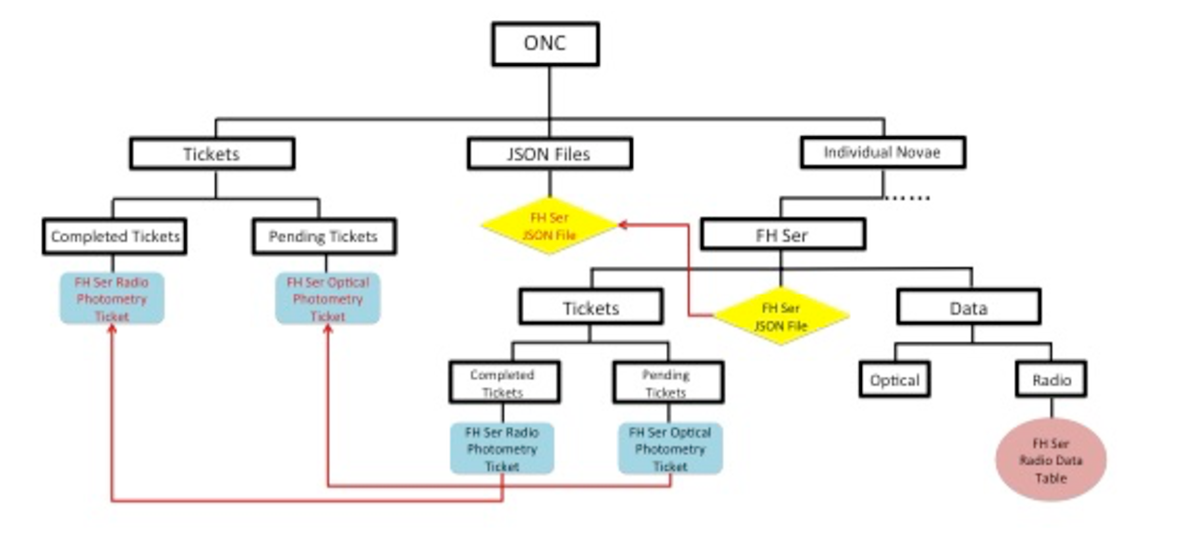
\includegraphics[width=15cm]{DataHierarchy_Pics/Pic6} 
%\caption{ }
%\label{fig:6}
\end{figure}

That's about it in terms of the data organization/hierarchy. Cheers!
\end{document}